\section{System Design}

\begin{figure}[t]
\centering
    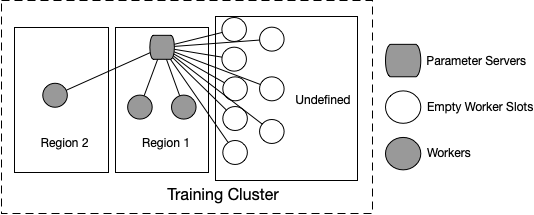
\includegraphics[width=\columnwidth ]{sparse_mapping.png}
\caption{\tian{placeholder} \textbf{\sysname architecture.} \sysname manages each training clusters and chooses the ``best'' configurations when the current GPU workers are revoked.}
    \label{design:spottrain}
\end{figure}

In this section, we describe how \sysname leverages our empirical measurement design to make the cluster management decisions about when and which cluster configurations to switch to. 

Considering $n$ different types of GPU servers, $G = \{G_1, \dots, G_n\}$, we keep track of lifetime $G_i^l$ for the $i^{th}$ type of GPU servers , which is defined as the time between $G_i
$ becomes available for cloud customers to start use, and the provisioning time $G_i^p$ (or $P_i$) as the time it takes between the user submits the request until the time the server becomes available. 
We also measure the revocation interval $G_i^r$ which captures the reliability of server $G_i$. 
For GCE, we can obtain a CDF that tells us the probability $P(G_i^p \leq t)$ that GPU $G_i^p$ the probability of being revoked in the next $t$ hours. (memoryless though?) We update the CDF with online usage data. 

The cluster $C_k$ is said to fail if and only if all the transient GPU servers have been revoked. Note that, the parameter server is running on an on-demand CPU server, and we have an evaluator that is shared by a number of GPU clusters. The evaluator is used to evaluate the current model’s accuracy and is needed regardless of whether we are using distributed training or single GPU training. 

Therefore, we can calculate the probability that $P(C_k fails) = \prod P(G_i^p \leq t)$ where $t$ is the total wall time of training the current model. 

\textbf{When to switch cluster configuration:} 
% 
We categorize cluster configuration changes into two types: voluntary and forced. Our goal in voluntary switch is to proactively figure out if any cluster configurations that are different from the current one is more beneficial for speeding up the training without violating the cost. Voluntary switch can happen in GCE when we predict the potential speedup of adding more GPU servers (or replacing existing slower GPU servers), and can also happen in EC2 when we observe cheaper GPU servers. The first one is termed as performance-driven voluntary switch and the latter one is defined as cost-driven voluntary switch. Note that the high level goal of voluntary switch is to eventually speed up training process. Forced switch can happen when cloud providers take away some or all transient servers from the same training clusters. It can happen in both cloud providers and is often followed with a voluntary switch to a better cluster configuration. In this paper, we focus on handling \emph{forced switch} (i.e., GCE) and leave voluntary switch for future work. 

\textbf{What cluster configuration to switch to:} 
% 
Simply picking the cheapest transient GPU servers is not enough. At the high level, this is because we also need to consider current cluster configurations, switch overhead, switching strategy, as well as the probability and the time interval to encounter the next force switch. That said, incorporating the cheapest GPU servers naively can lead to undesired training performance. 

Consider that the current cluster consists of a number of $K80$ servers in region one, and $P100$ servers in a different region becomes the cheapest. … 

Hmm, how about using a similarity metric to match the potential configuration to the existing configurations we keep track of, we then the existing performance profile as a proxy to approximate the training performance. Similarly, we already know the current cluster’s training performance, and we will only switch, if the potential configuration is significantly better (controlled by a threshold value) than the current configuration.  


%\subsection{TRANSIENT-SPECIFIC OPTIMIZATIONS}
\subsection{transient-specific optimizations}


Our measurements reveal XX key observations: 

(1)	When cheaper transient resources become available, it is better to split the risks by adding the transient resources in. To start, we will find the cheapest transient server and the most stable transient servers. 
(2)	current GPU transient servers have relative stable life time and we don’t need to aggressively checkpoint model. 
(3)	Utilizing intra region resources, i.e., by adding to the current cluster, if not done appropriately, can hurt distributed training performance. 

Based on each key observation, we propose a corresponding optimization technique and evaluate its effectiveness. 

Adaptively set the checkpoint frequency based on the lifetime measurement, and the model size. 

Reduce gradient update frequency when inter-cluster training is happening, and implement a gradient compression based on MXNet. 


Dynamically adjust the batch size given the current cluster configuration. The rationale is because a larger batch size, e.g., 1024 vs. 256 means fewer communication of weight gradients. This could be very useful if we perform intra-region training, because network can be very slow… However, as noted in [16] of FireCaffe, batch size has to be adjusted together with learning rate. For example, if we increase the batch size by 2x, we will also do so for the learning rate. 

Can we specify different batch sizes for different workers? So that we can reduce the communication between parameter servers and workers… and avoid the gradient update reach the parameter servers at the same time…


TensorFlow specific optimization. Because TensorFlow distributed training framework builds the model training computation graph at the beginning of the session, it does not support adding or removing workers during the training. To enable elastic scaling for TensorFlow, we propose to leverage a technique called sparse mapping, which allows us to add in up to $n$ number of workers after the training session is established. When a new worker becomes available, regardless whether it is within a region or outside a region, our \sysname will assign the worker with the pre-allocated IP address. The new worker can then start the training by performing mini-batch gradient computation, and communicate with the PS. (I am not quite sure how sparse mapping works.) In essence, it allows us to allocate virtual servers. An example setting of sparse mapping is shown in Figure~\ref{} with eleven virtual servers and three active workers and one active parameter server. More concretely, when initializing the training cluster, active servers will be supplied with cluster specifications with a total of eleven slots (of which only four are filled). 

\begin{figure}[t]
\centering
    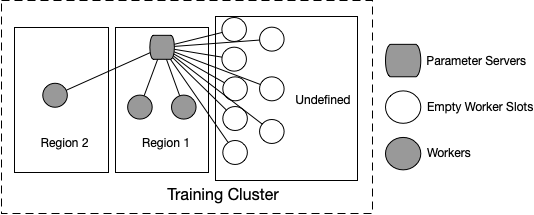
\includegraphics[width=\columnwidth ]{sparse_mapping.png}
\caption{\textbf{Elastic distributed training through sparse mapping.} By preallocating slots for virtual workers and adaptively adjusting learning rates, \sysname enables elastic distributed training without sacrificing training accuracy.}
    \label{design:sparse}
\end{figure}

